\chapter{Le moteur asynchrone}
\section{Principe de fonctionnement}
	\begin{wrapfigure}[10]{l}{4cm}
	\vspace{-5mm}
	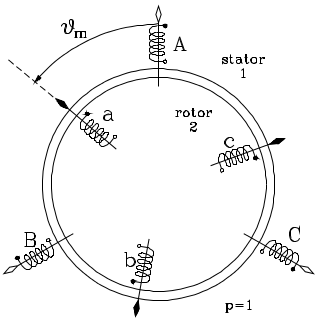
\includegraphics[scale=0.34]{ch5/image1.png}
	\captionof{figure}{ }
	\end{wrapfigure}
Alimentons les phases du stator\footnote{Analogue à celui d'une MS, Cf. ch7.} 
par une source de tension triphasée équilibrée d'ordre direct. Le rotor, lui, 
n'est relié à \textbf{aucune} source de tension (en fonctionnement normal, on 
parle de court-circuit) : il est fermé sur lui même. 
Le couple moteur résultera d'un champ tournant et on peut montrer que la vitesse 
de rotation du rotor $\Omega_r$ ne vaut jamais la vitesse de rotation du 
champ tournant statorique $\Omega_s$ ; \textbf{asynchrone}.\\

Ci-contre, $\vartheta_m$ représente l'angle entre le rotor et le stator. 


\section{Champs fixes et champs tournant}
	\subsection{Champ fixe}
	Comme pour la MCC, l'inducteur est dans le stator. Si la répartition de 
	l'induction est sinusoïdale dans l'entrefer, définissons le vecteur 
	spatial fixe $\vec{B}$ d'amplitude $B^M$ vaut le maximum d'induction, 
	c'est-à-dire l'orientation NS. L'induction au point $X$ repéré par la 
	coordonnée angulaire $\beta_m$ vaut
	\begin{equation}
	\begin{array}{ll}
	B_X &= B^M\cos(p\beta_m)\\
	&= B^M\cos\beta
	\end{array}
	\end{equation}
	\begin{center}
	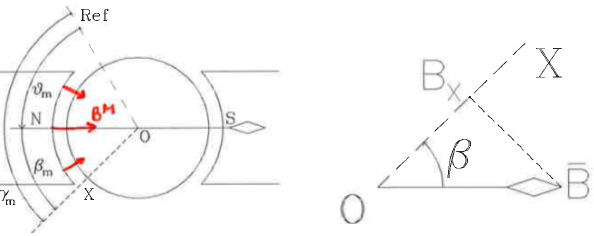
\includegraphics[scale=0.34]{ch5/image2.png}
	\captionof{figure}{ }
	\end{center}
	On multiplie l'angle par $p$ pour avoir l'angle électrique : $\beta_m = 
	\gamma_m-\vartheta_m$. Si $\beta_M \neq f(t)$, l'induction est constante 
	en chaque $X$. On peut alors obtenir la valeur de $B$ en $X$ décalé de 
	$\beta_M$ par rapport à l'axe NS par projection de $\vec{B}$ sur un axe 
	décallé $\beta = p\beta_m$.
	\newpage
	
	\subsection{Champ tournant - Conventions}
	\begin{wrapfigure}[11]{l}{4cm}
%	\vspace{-5mm}
	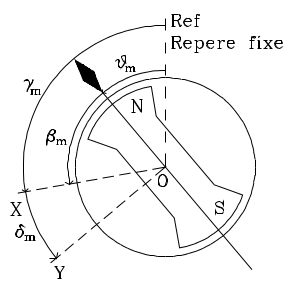
\includegraphics[scale=0.38]{ch5/image3.png}
	\captionof{figure}{ }
	\end{wrapfigure}
	Cette fois-ci, on définit un vecteur spatial $\vec{B}$ qui n'est plus fixe 
	mais \textbf{tournant} amenant la notion de champ sinusoïdal tournant. Par 
	contre le rotor voit un champ fixe, mais sinusoïdal dans l'espace. Notons 
	\begin{itemize}
	\item[$\bullet$] Le sens positif de rotation est le sens trigo.
	\item[$\bullet$] $\gamma_m$ repère $X$ par rapport à un axe statorique 
	fixe : coordonnée statorique.
	\item[$\bullet$] $\beta_m$ repère $X$ par rapport à l'axe $N$ de l'inducteur :
	coordonnée rotorique
	\item[$\bullet$] $\beta_m$ repère l'axe $N$ de l'inducteur par rapport à 
	l'axe statorique de référence.
	\item[$\bullet$] Induction $N \rightarrow S$ est positive.		
	\end{itemize}
	
	
	\subsection{Induction en un point fixe $X$}
	Comme précédemment, si la répartition spatiale de l'induction est sinusoïdale, 
	sa valeur en $X$ vaut 
	\begin{equation}
	B_X = B^M\cos(p\beta_m) = B^M\cos\beta
	\end{equation}
	sauf qu'ici, $\beta_m \neq\ cste$. Si le rotor tourne à vitesse constante 
	$\Omega_r$ :
	\begin{equation}
	\theta_m = \Omega_rt + \theta_{m0}\quad \text{où } \theta_{m0}\ \text{ est 
	la position du rotor en $t=0$}
	\end{equation}
	On a donc
	\begin{equation}
	\theta = p\theta_m = p\Omega_rt + p\theta_{m0} = \omega t +\theta_0
	\end{equation}
	où $\omega = p\Omega_r, \theta_0=p\theta_{m0}$. Jouons avec les phaseurs 
	et nos deux angles $\theta, \gamma$ défini ci-dessus\footnote{Pq $-\gamma$?} :
	\begin{equation}
	\begin{array}{lll}
	B_X &= \Re(\vec{B}.\vec{1_x}^*) &= \Re(B^M\ e^{j(\theta-\gamma)})\\
	&= \Re(B^M\ e^{j(\omega t + \theta_0-\gamma)}) &= B^M\cos(\omega t+\theta_0
	-\gamma)
	\end{array}
	\end{equation}
	Le champ $B_x$ varie donc sinusoïdalement dans le temps. On peut encore 
	l'écrire 
	\begin{equation}
	B_X = \Re(B^M\ e^{j(\theta_0-\gamma)}\ e^{j\omega t}) \equiv \Re(\underline{B}
	\sqrt{2}\ e^{j\omega t})
	\end{equation}
	avec 
	\begin{equation}
	\underline{B} = \dfrac{B^M}{\sqrt{2}}\ e^{j(\theta_0-\gamma)}
	\end{equation}
	

	Un observateur rotorique verra une répartition spatiale de l'induction alors 
	qu'un observateur statorique (fixe) voit passer un champ tournant. Un 
	observateur statorique placé à un autre endroit voit le même champ tournant, 
	de même amplitude mais déphasé. L'illustration ci-dessus montre deux moyens 
	d'obtenir $B_X$ et $B_Y$.
	\begin{center}
	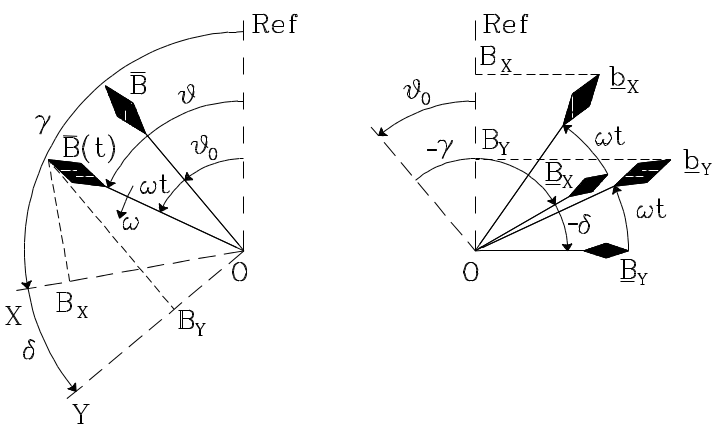
\includegraphics[scale=0.34]{ch5/image4.png}
	\captionof{figure}{Ces deux représentations donnent les mêmes infos : l'une est 
	un champ qui tourne "physiquement" et l'autre est repris en phaseurs.}
	\end{center}
	

\section{Les f.e.m. engendrées dans les enroulements ouverts}
	\subsection{Étoiles des encoches}
		\begin{wrapfigure}[11]{l}{10cm}
	\vspace{-5mm}
	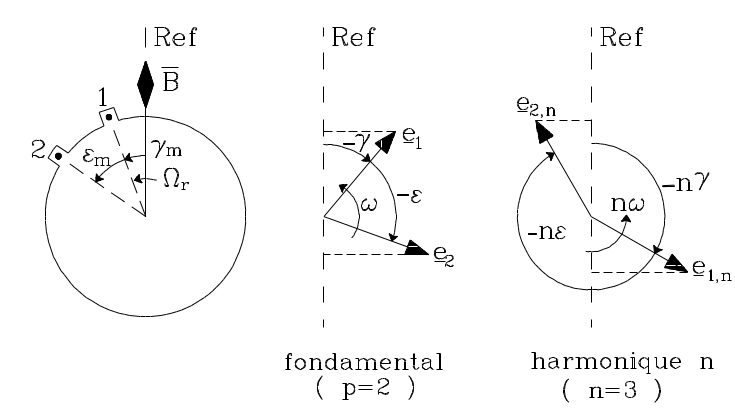
\includegraphics[scale=0.38]{ch5/image5.png}
	\captionof{figure}{ }
	\end{wrapfigure}
	Le calcule des phaseurs de tension pour un conducteur 1, décalé de 
	$\gamma_m$ s'obtient via $e= Blv$.\\
			1 et 2 sont deux conducteurs fixes dans des encoches. $\Omega_r$ 
	est la vitesse de rotation mécanique. Comme $e=Blv$, la tension $\propto B \rightarrow$ 
	les phaseurs de $B$ et $e$ ont la même direction. Le $-\epsilon$ signifie que $e_2$ 
	est en retard par rapport à $e_1$.\\
	

	\subsection{Étoiles des bobines - Raccourcissement du pas}
	Soit une spire composée d'un conducteur aller 1 et retour 1'. Si les spires sont 
	diamétrales (électriquement opposé, $\angle 11' = \pi/p$), la tension à ses bornes 
	est simple : $e_{(1)} = e_1-e_{1'}$.
	\begin{center}
	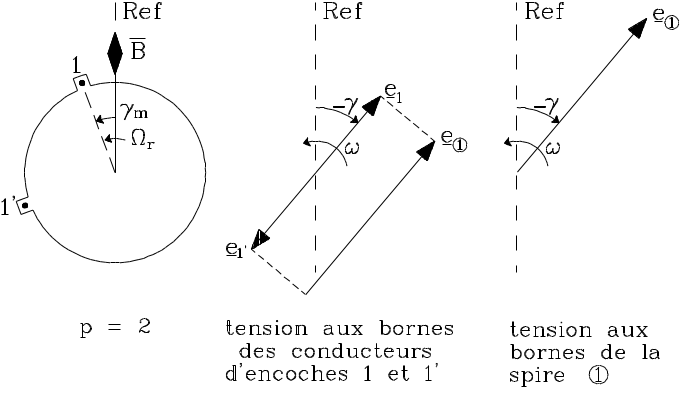
\includegraphics[scale=0.38]{ch5/image6.png}
	\captionof{figure}{ }
	\end{center}
	
	\newpage	
	Si la spire (11') n'est \textbf{pas} diamétrale, les choses changent. Considérons 
	le conducteur 1" tel que la spore 11" soit diamétrale : la tension en 1' est 
	déphasée de $np\delta m=n\delta$ par rapport à celle en 1" valant l'opposé de celle 
	en 1. La f.e.m. $e_{(1)}=e_1-e_{1'}$ est décalée de $n\delta/2$ par rapport à $e_1$.\\
	
	\begin{wrapfigure}[11]{l}{9cm}
	\vspace{-5mm}
	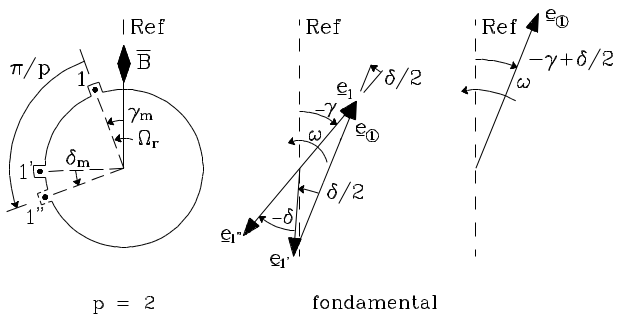
\includegraphics[scale=0.38]{ch5/image7.png}
	\captionof{figure}{ }
	\end{wrapfigure}
	Dû au raccourcissement du pas $\delta_m$, l'amplitude est inférieur à $2*e_1$. La 
	phase est donc identique à celle d'une spire \textbf{diamétrale} de même axe que 
	la spire 11'. Cette spire diamétrale équivalente est décalée d'un angle mécanique 
	négatif $-\delta_m/2$ par rapport à 1 et d'un angle mécanique positif $\delta_m/2$ 
	par rapport à 1'. On peut alors calculer la f.e.m. dans la spire réelle en multipliant 
	la f.e.m. de la spire diamétrale équivalente par le \textbf{facteur de raccourcissement 
	de pas }
	\begin{equation}
	k_R = \cos\dfrac{n\delta}{2}=\cos\dfrac{np\delta_m}{2}
	\end{equation}
	où $n$ est le numéro de l'harmonique.
	
	\subsection{Étalage des encoches}
	\begin{wrapfigure}[11]{r}{9cm}
	\vspace{-8mm}
	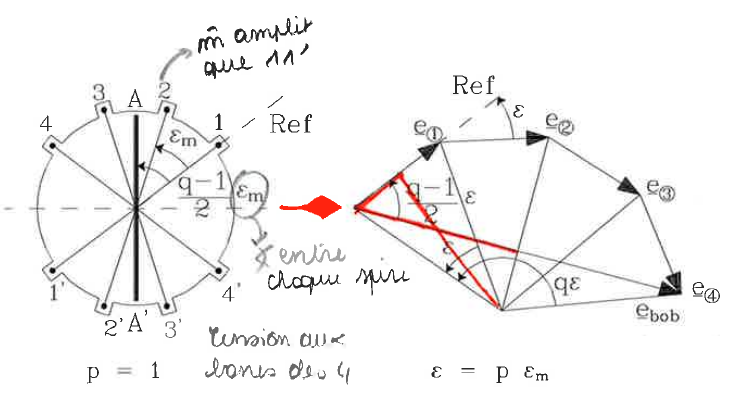
\includegraphics[scale=0.38]{ch5/image8.png}
	\captionof{figure}{ }
	\end{wrapfigure}
	On considère maintenant $q$ spires diamétrales en séries décalée d'un angle mécanique
	$\epsilon_m$ l'une par rapport à l'autre. Toutes les spires (22',33',\dots) ont la 
	même amplitude que 11'. Vu qu'elles sont en série, on prend la tension aux bornes des 
	(ici) quatre spires, les tensions vont s'additionner mais la tension totale ne vaudra 
	pas quatre fois celle de la spire 11' : facteur de diminution. On l'appelle le 
	\textbf{facteur d'étalage} que l'on peut calculer avec la règle des sinus :
	\begin{equation}
	k_E = \dfrac{\sin\left(\dfrac{nq\epsilon}{2}\right)}{q\sin\left(\dfrac{n\epsilon}{2}
	\right)}
	\end{equation}
	
	\subsection{Obliquité des encoches}
	Si les encoches sont \textit{un peu de travers}, l'amplitude de la tension réelle 
	est obtenue en multipliant la tension aux bornes du conducteur par le \textbf{facteur 
	d'obliquité }:
	\begin{equation}
	k_0 = \dfrac{\sin np/2}{np/2}
	\end{equation}
	On peut utiliser cette technique pour supprimer les harmoniques des dentures.
	
	\subsection{Tension aux bornes d'une bobine}
	"\textit{En résumé, la tension aux bornes d'une bobine est obtenue en multipliant la 
	tension aux bornes d'une bobine constituée d'un même nombre de spires diamétrales dont 
	l'axe est celui de la bobine réelle, par le produit des facteurs d'obliquité, d'étalage 
	et de raccourcissement de pas.}"
	
	
\section{Champ magnétique et inductance dans la machine linéaire à entrefer constant}
On cherche à obtenir les coefficients d'inductance propre et mutuelles entre les enroulements 
comme pour le transformateur.

	\subsection{Force magnétomotrice dans une machine à entrefer constant}
		\begin{wrapfigure}[11]{r}{5cm}
	\vspace{-5mm}
	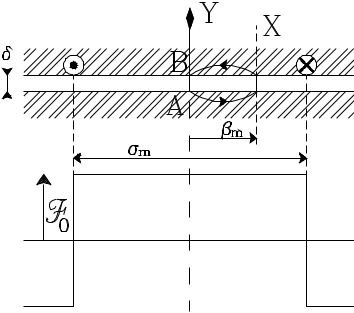
\includegraphics[scale=0.38]{ch5/image9.png}
	\captionof{figure}{ }
	\end{wrapfigure}
	Soit une bobine d'axe $Y$ avec $N_1$ spires confondues. La largueur (angulaire) de 
	ces spires vaut $\sigma_m$. On repère le point $X$ par sa coordonnée $\beta_m$ par 
	rapport à l'axe de la bobine. La différence de potentiel magnétique entre stator 
	et rotor dans l'axe $A-B$ vaut 
	\begin{equation}
	\Delta V_0 = H_{(0)}\delta \equiv \mathcal{F}_0
	\end{equation}
	souvent dit \textit{force magnétomotrice} $\mathcal{F}_0$ par abus de langage. Par 
	convention la f.m.m. au point $X$ ($\mathcal{F}_{(\beta m)}$ désigne la f.m.m. entre 
	les points $A$ et $B$ le long d'un chemin traversant l'entrefer au point $X$. La loi 
	des f.m.m. donne (Ampère)\footnote{??} :
	\begin{equation}
	\begin{array}{ll}
	\mathcal{F}_{(\beta m)} - \mathcal{F}_0 &= 0  \text{ si } |\beta_m|<\sigma_m/2\\
	&= -Ni  \text{ si } |\beta_m|>\sigma_m/2
	\end{array}
	\end{equation}
	Par symétrie, $\mathcal{F}_0 = Ni/2$. Si le fer est parfait et l'entrefer constant, 
	le champ magnétique vaut 
	\begin{equation}
	\begin{array}{ll}
	H_{(\beta m)} &= \dfrac{Ni}{2\delta}\ \text{ si }\ |\beta_m|<\sigma_m/2\\
	&= -\dfrac{Ni}{2\delta}\ \text{ si }\ |\beta_m|>\sigma_m/2
	\end{array}
	\end{equation}
	et l'induction
	\begin{equation}
	B_{(\beta m)} = \mu_0H_{(\beta_m)}
	\end{equation}
	La figure ci-dessous représente l'effet de bobines concentriques à même nombre de 
	spires parcourues par le même courant. On voit que cela ressemble fortement à un 
	beau sinus
	\begin{center}
	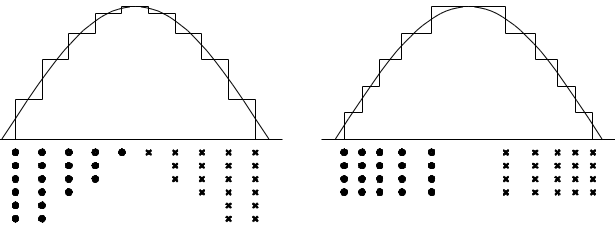
\includegraphics[scale=0.38]{ch5/image10.png}
	\captionof{figure}{ }
	\end{center}
	
	\subsection{Titre beaucoup trop long}
	Pour une sous-section dont il a seulement dit quelque chose ?
	
	\newpage
	\subsection{Facteurs d'étalage, de raccourcissement, d'obliquité}
	\begin{wrapfigure}[8]{l}{9cm}
	\vspace{-5mm}
	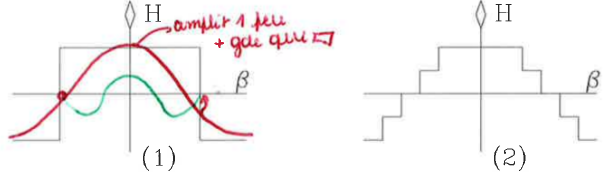
\includegraphics[scale=0.38]{ch5/image11.png}
	\captionof{figure}{ }
	\end{wrapfigure}
	Ci-contre, à gauche quatre spire diamétrales et à droite quatre spires 
	étalées. En configuration étalée, le champ est bien plus sinusoïdal et il peut 
	l'être complètement avec un choix judicieux (hypothèse pour le reste du cursus).\\

	Limité à son fondamental, le champ à pour expression
	\begin{equation}
	H_{(\beta)} = k_Ek_Rk_O\dfrac{N_fi_f}{2\delta p}\dfrac{4}{\pi}\cos\beta
	\end{equation}
	Dans un cas \textit{confondu}, $N_f/p$ représente les spires en dessous de la 
	première paire de pôle. Dans le cas \textit{réparti}, on ne prend plus que le 
	fondamental. Le facteur de "correction rectangle" pour n'obtenir que le fondamental 
	est $4/\pi$. Après, les facteurs d'obliquité, \dots sont présents pour effectuer 
	les différentes corrections.\\
	Pour rendre ça tout smooth, on défini le \textbf{nombre effectif de spires}
	\begin{equation}
	N_{sf} \equiv \dfrac{4}{\pi}k_Ek_Rk_ON_f
	\end{equation}
	Ce nombre de spire donne le même "fondamental". On peut alors écrire
	\begin{equation}
	H_{(\beta)} = \dfrac{N_{sf}i_f}{2\delta p}\cos\beta
	\end{equation}
	On note aussi souvent $k_f=k_ek_Rk_O$ pour rendre ça $e^{\text{smooth}}$.
	
	
	\subsection{Inductance propre d'une bobine dans une machine à entrefer constant}
	\begin{wrapfigure}[8]{l}{5cm}
	\vspace{-8mm}
	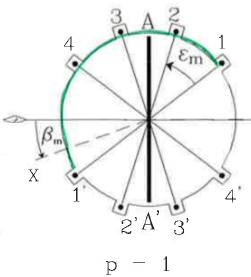
\includegraphics[scale=0.45]{ch5/image12.png}
	\captionof{figure}{ }
	\end{wrapfigure}
	Soit $q$ spires décalées de $\epsilon_m$ l'une de l'autre. Avec le courant $i_f$, 
	le \textbf{fondamental} du champ vaut au point $X$ de coordonnée $\beta_m$ :
	\begin{equation}
	H_{(\beta)} = k_E\dfrac{N_fi_f}{2\delta p}\dfrac{4}{\pi}\cos\beta
	\end{equation}
	L'induction se déduit directement : $B_{(\beta)} = \mu_0H_{(\beta)}$. Le flux 
	coupé par la spire (1) vaut \\
	\ \\
	
	\begin{equation}
	\Phi_{(1)} = \int_{-\frac{\pi}{2p}-\frac{q-1}{2}\epsilon_m}^{\frac{\pi}{2p}-
	\frac{q-1}{2}\epsilon_m} B_{(\beta_m)} lRd\beta_m = \dfrac{\mu_0lR}{p^2\delta}
	\left(\dfrac{4}{\pi}k_EN_f\right)i_f\cos\dfrac{q-1}{2}\epsilon
	\end{equation}
	On peut voir $\Phi_{(1)}$ comme la valeur de la projection de la spire du flux
	$\Phi_\perp$ coupé par une spire identique mais dont l'axe serait celui de la 
	bobine \textbf{ou} le flux coupé par la spire diamétrale après qu'on ai 
	inversé les axes de la bobine et de la spire.
	\begin{equation}
	"\ \Phi_\perp \cos\dfrac{q-1}{2}\epsilon\ "
	\end{equation}
	
	\begin{center}
	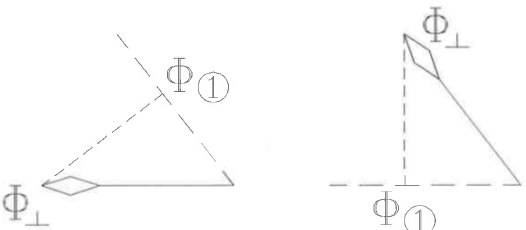
\includegraphics[scale=0.45]{ch5/image13.png}
	\captionof{figure}{ }
	\end{center}
	On a alors
	\begin{equation}
	\Phi_\perp = \dfrac{\mu_0lR}{p^2\delta}\left(\dfrac{4}{\pi}k_EN_f\right)i_f
	\end{equation}
	Ceci est le flux dans une des spires. L'avantage c'est que maintenant on peut 
	tout sommer brutalement, même les spires qui ne sont pas dans la même direction!\\
	
	\begin{wrapfigure}[7]{r}{5cm}
	\vspace{-8mm}
	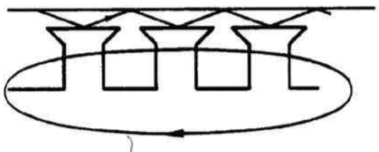
\includegraphics[scale=0.45]{ch5/image14.png}
	\captionof{figure}{ }
	\end{wrapfigure}
	Le flux totalisé pour $N_f/p$ spires d'une paire de pôles s'obtient comme on 
	l'avait fait avant, en tenant compte de $k_E$ :
	\begin{equation}
	\Psi_{\text{2 pôles}} = k_E\dfrac{N_f}{p}\Phi_\perp = \dfrac{1}{p}(k_EN_f)
	\dfrac{\mu_0}{p^2\delta}lR\left(\dfrac{4}{\pi}k_EN_f\right)i_f
	\end{equation}
	Et donc pour $p$ paires de pôles :
	\begin{equation}
	\Psi = \left(\dfrac{4}{\pi}k_EN_f\right)^2\dfrac{\pi}{4}\dfrac{\mu_0lR}{p^2\delta}
	i_f
	\end{equation}
	On peut faire le même raisonnement avec $k_O$ et $k_R$. On obtiendrait alors :
	\begin{equation}
	\Psi = i_fN_{sf}^2\mathcal{P}_m
	\end{equation}
	où $N_{sf}$ est le nombre effectif de spires et $\mathcal{P}_m$ est la perméance 
	du circuit magnétique (mise en série de $2p$ entrefers). Ceci ne concerne que 
	la flux dans l’entrefer (flux utile, commun) sans le traverser (le flux reste 
	dans le stator). \\
	On en déduit l'inductance \textbf{linéaire} de la bobine pour le fondamental du 
	champ
	\begin{equation}
	L_f = l_f + N_{sf}^2\mathcal{P}_m
	\end{equation}
	Expression semblables à celle des transfo et non-influencée par la position du
	rotor.
	
	
	\subsection{Inductance mutuelle entre une bobine statorique et une bobine rotorique 
	dans une machine à entrefer constant}
	Soit un enroulement statorique $A$ et un rotorique $f$ dont les axes sont 
	décalés de $\chi$. Il faut suivre un raisonnement similaire au chapitre précédent. 
	Le flux coupé par une spire diamétrale d'axe $f$ pour un courant statorique $i_a$ 
	vaut
	\begin{equation}
	\Phi_\chi = \Phi_\perp\cos\chi
	\end{equation}
	Rebelote (après quelques calculs) :
	\begin{equation}
	\Psi_{fA} = l_fN_f\Phi_\chi =  i_AN_{sf}N_{sA}\mathcal{P}_m\cos\chi
	\end{equation}
	On trouve que le flux d'entrefer (commun) créé et 	coupé par $A$ vaut 
	\begin{equation}
	\Psi_{AA} = i_AN_{sA}^2\mathcal{P}_m
	\end{equation}
	L'expression de la mutuelle entre les deux enroulements est alors
	\begin{equation}
	M_{fA} = N_{sf}N_{sA}\mathcal{P}_m\cos\chi
	\end{equation}
	où les $N_i$ représentent les nombres de spires rotor/stator, $\mathcal{P}_m$ 
	est nécessaire car les flux traversent l'entrefer, $\chi$ est l'angle 
	électrique si l'on a $p$ paires de pôles et la présence du $\cos$ intervient 
	alors lorsque ceux-ci ne sont pas alignés.
	
	\subsection{Inductance mutuelle entre deux bobines statoriques dans une machine 
	à entrefer constant}	
	On peut déduire cette expression dans un systèmes triphasé avec la formule 
	précédente, si $\chi=2\pi/3$. Il faut cependant rajouter un terme supplémentaire 
	provenant du flux de dispersion d'une phase qui, même s'il ne traverse pas 
	l'entrefer, arrive à l'autre phase :
	\begin{equation}
	M_{AB} = l_A'+N_1^2\mathcal{P}_m\cos\dfrac{2\pi}{3} = l_A'-\dfrac{1}{2}N_1^2
	\mathcal{P}_m
	\end{equation}
	On obtient des expressions semblables pour le rotor.
	
	\subsection{Matrice des coefficients d'inductance pour une machine linéaire à 
	entrefer constant comportant 3 enroulement $ABC$ au stator et 3 enroulement 
	$abc$ au rotor}
	\begin{wrapfigure}[11]{r}{4cm}
	\vspace{-8mm}
	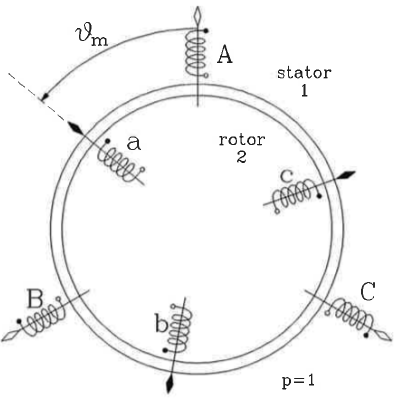
\includegraphics[scale=0.3]{ch5/image15.png}
	\captionof{figure}{ }
	\end{wrapfigure}
	La page 5.28 reprends la définition des différentes phases, il faut ensuite 
	tout injecter dans une matrice beaucoup trop grande pour que je la  mette ici. 
	Rien de compliquer, c'est vraiment appliquer les formules trouvées plus haut.\\
	
	A l'examen, on peut demander un moyen de calculer les inductances via différents 
	nombre de spires effectives et des facteurs d'états,\dots\\
	
	On obtient une belle matrice d'inductances qui permet de calculer tous les flux 
	en fonction des courants (et pleins de paramètres, évidemment). Rappelons que 
	pour avoir un sens, il ne faut pas prendre en tête les  hypothèses suivantes:
	\begin{enumerate}
	\item Harmoniques spatiaux de $B,H$ et de la f.m.m. négligés
	\item Entrefer constant
	\item Non-linéarités magnétiques négligées
	\end{enumerate}
	De plus, ces expression sont valables en valeurs \textbf{instantanées}.
	
	
	\newpage
\section{Champs pulsant et champs tournants}
	\subsection{Les champs créés par une bobine unique}
	La f.m.m. d'une bobine d'axe $f$ parcouru par un courant $i_f$ réduit à son 
	fondamental vaut (on reprend les notations précédemment définies)
	\begin{equation}
	\mathcal{F}_{(\beta)} = \dfrac{N_fi_f}{2p}\dfrac{4}{\pi}\cos\beta
	\end{equation}
	Le vecteur $\vec{\mathcal{F}}$ est aligné selon l'axe électrique de la bobine. 
	Rappelons que le facteur $4/\pi$ vient des spires diamétrales (la surface étant 
	de ce facteur plus grand que le cas rectangulaire)
	Son amplitude vaut 
	\begin{equation}
	\mathcal{F}^M = \dfrac{N_fi_f}{2p}\dfrac{4}{\pi}
	\end{equation}
	$\mathcal{F}^M \propto$ valeur \textbf{instantanée} de $i_f$. On définit alors 
	un \textbf{vecteur} courant $\vec{i_f} = i_fe^{i\theta}$



		\subsection{Cas particuliers}
			\begin{wrapfigure}[11]{r}{4cm}
	\vspace{-8mm}
	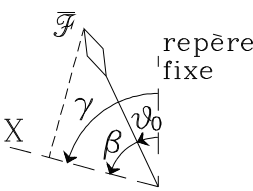
\includegraphics[scale=0.5]{ch5/image16.png}
	\captionof{figure}{ }
	\end{wrapfigure}
		$\triangleright$ Si la bobine est \textbf{fixe} et le courant \textbf{constant} 
		alors f.m.m. est constante dans le temps et se réparti sinusoïdalement. On trouve 
		la valeur de cette f.m.m. en un point $X$ par projection de $\vec{\mathcal{F}}$ 
		sur $OX$.\\
		Avec $\vec{\mathcal{F}}$ et $\vec{i_f}$, on trouve :
		\begin{equation}
		\mathcal{F}_{(x)} = \Re(\vec{\mathcal{F}}.\vec{1_X}^*) = \mathcal{F}^M\cos(
		\theta_0-\gamma)
		\end{equation}
		On peut voir cette projection comme la f.m.m. consommée en ce point.\\
		
		
		$\triangleright$ Si la bobine est \textbf{tournante} et le courant est 
		\textbf{constant}, la f.m.m. est dite \textbf{tournante}. Nous avons 
		cette fois-ci :
		\begin{equation}
		\vec{\mathcal{F}} = \frac{4}{\pi}\dfrac{N_fi_f}{2p}e^{j(\omega_rt+\theta_0)}, 
		\qquad \vec{i_f} = i_fe^{j(\omega_rt+\theta_0)}
		\end{equation}
		Au point $X$, notre f.m.m sera sinusoïdale dans le temps (normal, vu que ça 
		tourne), de pulsation $\omega_r$.
		\begin{equation}
		\mathcal{F}_{(X)} = \mathcal{F}^M\cos(\omega_rt+\theta_0-\gamma)
		\end{equation}\ \\
		
				
		$\triangleright$ Si la bobine est \textbf{fixe} et le courant est 
		\textbf{sinusoïdal} $i_f = I_{Mf}\cos(\omega t+\xi_f)$, la f.m.m. est 
		dite \textbf{pulsante} et, à chaque endroit, elle est sinusoïdale dans 
		le temps\footnote{??}.\\
		
		En développant les calculs on peut montrer que \textit{tout champ pulsant 
		est la somme de deux champs tournants de même amplitude, de même vitesse 
		mais de sens contraire. Celui dans le sens positif est dit "direct" et 
		"indirect pour l'autre". Leur amplitude vaut la moitié de celle du champ 
		pulsant. Leurs vitesse de rotation est celle du courant}.\\
		
		Pour la machine synchrone, nous allons réaliser un stator à trois enroulements 
		parcouru par un courant triphasé. Chacune des bobines crée un champ pulsant. 
		La recombinaison de ces trois champs donne un champ tournant.
		
\newpage		
\section{La machine asynchrone à rotor bobiné en régime}
En régime équilibré, la somme des courants est nulle à tout instant. En développant 
la masta-matrice vue plus haut, le flux totalisé se compose de trois termes :
\begin{equation}
\Psi_A = l_1i_A + \dfrac{3}{2}N_1^2\mathcal{P}_mi_a + M^M[\dots]
\end{equation}
Le premier terme est le flux de dispersion, le second le flux commun d'entrefer dû 
au stator et le dernier le flux commun d'entrefer dû au rotor.

	\subsection{Alimentation symétrique d'ordre direct - machine à l’arrêt}
		\subsubsection{Alimentation par le stator - rotor ouvert}
		Le stator est alimenté par un système de trois tension équilibré et 
		comme le rotor est ouvert $i_2=0 (=i_a=i_b=i_c)$. On obtient alors
		\begin{equation}
		\begin{array}{ll}
		\Psi_A &= l_1i_A + \frac{3}{2}N_1^2\mathcal{P}_mi_A\\
		v_a &= r_1i_A + (l_1+\frac{3}{2}N_1^2\mathcal{P}_m)\frac{di_a}{dt}
		\end{array}
		\end{equation}
					\begin{wrapfigure}[15]{r}{5cm}
	\vspace{-8mm}
	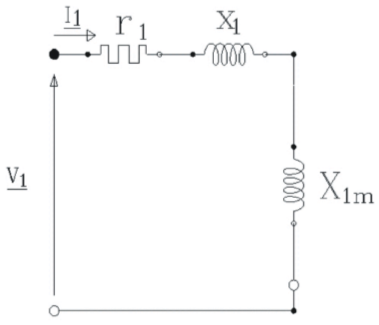
\includegraphics[scale=0.5]{ch5/image17.png}
	\captionof{figure}{ }
	\end{wrapfigure}
		Comme nous avons un système de tensions équilibrés au stator, il circule
		un système de tensions équilibrés d'ordre direct au stator:
		\begin{equation}
		\underline{V_1} = (r_1+j\omega l_1)\underline{I_1}+j(\omega\frac{3}{2}
		N_1^2\mathcal{P})\underline{I_1}
		\end{equation}
		avec $\underline{V_1}$ le phaseur de la composante directe de tension, 
		$\underline{I_1}$ le phaseur de la composante directe de courant, 
		$x_1=\omega l_1$ la réactance de dispersion statorique. En définissant 
		$\underline{z_1} = r_1+jx_1$ et $X_{lm} = 3/2\omega N_1^2P_m$ la 
		réactance de magnétisation statorique (dont la valeur dépend de l'état 
		magnétique), on peut écrire
		\begin{equation}
		\underline{V_1} = (r_1+jx_1)\underline{I_1}+jX_{1m}\underline{I_1}
		\end{equation}
		conduisant au schéma équivalent ci-contre.\\
		
		La phaseur de la composante directe du \textbf{flux rotorique} vaut 
		\begin{equation}
		\underline{\Psi_2}=M^M[\underline{I_A}\cos\theta + \underline{I_B}
		\cos(\theta-\frac{2\pi}{3}) + \underline{I_C}\cos(\theta+\frac{2\pi}{3})]
		\end{equation}
		En explicitant les phaseurs du courant en fonction de $\underline{I_A}$ 
		et en exprimant les cosinus grâce aux exponentielles complexes (détail 
		page 5.43) on peut écrire
		\begin{equation}
		\underline{\Psi_2} = \dfrac{3}{2}N_1N_2\mathcal{P}_m\underline{I_1}e^{-j
		\theta}
		\end{equation}
		La tension appliquée au rotor vaut donc
		\begin{equation}
		\begin{array}{ll}
		\underline{V_2} = j\omega\underline{\Psi_2} = j\omega\dfrac{3}{2}N_1N_2
		\mathcal{P}_m\underline{I_1}e^{-j\theta}\\
		&= j\left[\dfrac{N_2}{N_1}\right]X_{1m}\underline{I_1}e^{-j\theta}
		\end{array}
		\end{equation}
		Posons $\mu = N_1/N_2$ le rapport de transformation stator-rotor. On a 
		donc, comme pour les transfo :
		\begin{equation}
		\mu\underline{V_2} = jX_{1m}\underline{I_1}e^{-j\theta}
		\end{equation}
		\newpage
		\begin{wrapfigure}[10]{l}{9cm}
		\vspace{-8mm}
		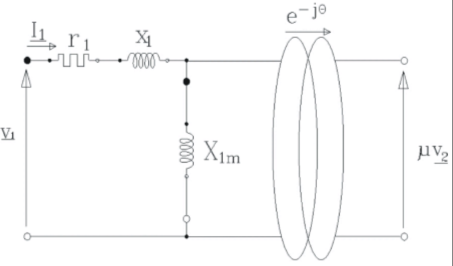
\includegraphics[scale=0.5]{ch5/image18.png}
		\captionof{figure}{ }
		\end{wrapfigure}
		On obtient alors le schéma équivalent d'une machine d'induction à l'arrêt, 
		rotor ouvert. On voit que le champ tournant induit au rotor un système 
		symétrique de tension \textbf{déphasée en arrière} de $\theta$ car la phase 
		$a$ du rotor est décalée en avant de $\theta_m$ par rapport à la phase $A$ 
		du stator.\\
		
		
		
		\subsubsection{Alimentation par le rotor - Stator ouvert}		
		Ici, le rotor crée un champ tournant et la tension est induite dans le 
		stator (qui ne tourne bien évidemment pas). On obtient exactement le 
		schéma, mais dans l'autre sens : $-\theta\rightarrow\theta, 1\rightarrow 2,
		\mu \rightarrow 1/\mu$. Par un raisonnement identique, on obtient le 
		schéma équivalent dans lequel on trouve
		\begin{equation}
		X_{2m} = \frac{3}{2}\omega N_2^2\mathcal{P}_m = \dfrac{X_{1m}}{\mu^2}
		\end{equation}
		\begin{center}
		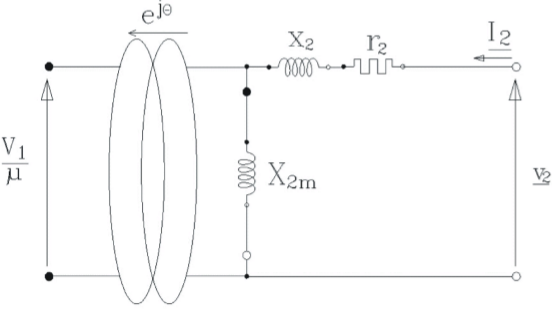
\includegraphics[scale=0.5]{ch5/image19.png}
		\captionof{figure}{ }
		\end{center}
		avec $X_2$ la réactance de dispersion, $r_2$ la résistance de la bobine 2, 
		$X_{2m}$ la réactance de magnétisation. On peut transformer ce schéma en 
		multipliant les tensions par $\mu$, les courants par $1/\mu$, les impédances 
		par $\mu^2$ et en inversant le sens du déphaseur
		\begin{center}
		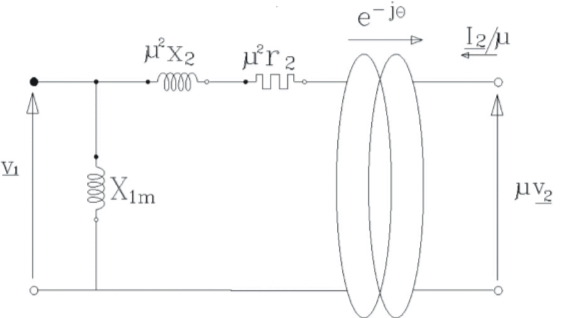
\includegraphics[scale=0.5]{ch5/image20.png}
		\captionof{figure}{ }
		\end{center}		
		
		\newpage
		\subsubsection{Alimentation par le stator et le rotor}
		Le schéma équivalent d'une machine d'induction \textbf{à l’arrêt} s'obtient 
		en superposant l'effet des courants statoriques et rotoriques. Il va falloir 
		procéder à une mise à échelle. En effet $X_{1m} = N_1^2\mathcal{P}_m \neq 
		X_{2m} = N_2^2\mathcal{P}_m$ (l'une restant en grande partie dans le stator). 
		Pour mettre à l'échelle, on retrouve notre $\mu^2$ pour les impédances, 
		le $\mu$ pour les tensions et le $1/\mu$ pour le courant. Le schéma ci-dessous
		est très semblable à celui d'un transformateur
		
		\begin{center}
		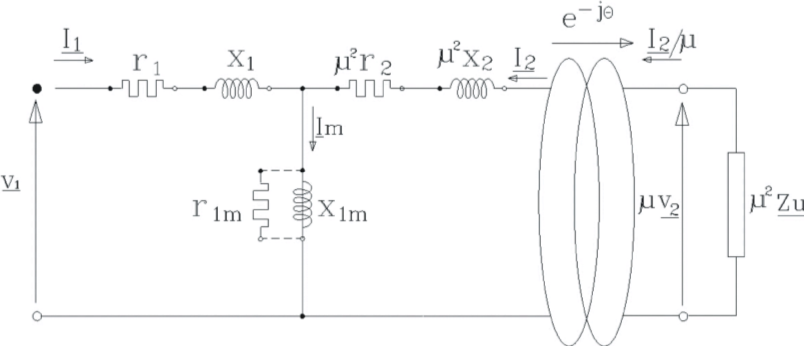
\includegraphics[scale=0.5]{ch5/image21.png}
		\captionof{figure}{ }
		\end{center}		
		Notons que la réactance de magnétisation est beaucoup plus faible ici que 
		dans le transformateur (dû au grand entrefer dans le transfo). Sur notre 
		schéma équivalent, deux flux tournants vont s'additionner et on obtiendra 
		le flux commun dans l'entrefer.  Ce flux commun passe par le fer du rotor 
		et du stator, il subit des pertes par hystérèses et courants de Foucault 
		(représenté par la résistance mise en parallèle).\\
		On a créé ici le circuit parfait pour déphasé du triphasé.
		
		\subsubsection{Couple à l’arrêt}
		Soit les résistances/réactances statoriques ($r_1,x_1=0$) négligeables et
		le rotor en court-circuit. Si on applique $\underline{V_1}$, cela va induire 
		dans le rotor un courant déphasé en arrière par rapport à $\underline{V_1}$. 
		Ces courants rotoriques, couplés au champ tournant, créent un couple.
		
		
	\subsection{Alimentation symétrique d'ordre direct - machine en rotation imposée 
	par l'extérieur}
		\subsubsection{Alimentation par le stator - Rotor ouvert}
		Comme les courants rotoriques sont nuls (rotor ouvert) il  n'y a pas de couple 
		moteur. Entraînons le rotor à la vitesse $\Omega_r$. Par rapport au rotor, le 
		champ tourne à vitesse \textbf{électrique} $= <-p\Omega_R = \omega-\omega_r$. 
		Les tensions engendrée au rotor on une pulsation $\omega-\omega_r$.\\		
		On définit le \textbf{glissement} de la façon suivante :
		\begin{equation}
		g = \dfrac{\omega-\omega_R}{\omega}
		\end{equation}
		où $\omega_R$ est la vitesse de rotation électrique. Si celui-ci vaut 1, 
		la machine est à l'arrêt. S'il est nul, c'est qu'il n'y a plus de tension 
		dans la bobine. S'il vaut 2, le rotor tourne à la même vitesse que le champ 
		tournant mais en sens inverse. En général, $g$ est petit. Ce facteur exprime 
		que le rotor tourne un peu en arrière par rapport au champ généra d’où 
		l'asynchronisme.\\
		
		Le calcul de $\Psi_1$ est identique au cas précédent (où le rotor était à 
		l'arrêt): la rotation du rotor ne change rien.Le schéma équivalent est donc 
		le même.\\

		Pour $\Psi_2$ :
		\begin{equation}
		\underline{\Psi_2} = \frac{3}{2}N_1N_2\mathcal{P}_m\underline{i_1}e^{-j\theta} 
		= \dfrac{X_{1m}}{\mu\omega}\underline{i_1}e^{-j\theta}
		\end{equation}
		C'est ici que les choses changent. Nous avons en effet
		\begin{equation}
		\begin{array}{ll}
		\theta &= \theta_0 + \omega_rt\\
		\underline{i_1} &= I_1\sqrt{2}e^{j(\omega t+\xi_I)}
		\end{array}
		\end{equation}
		Il en vient que
		\begin{equation}
		\underline{\Psi_2} = \dfrac{X_{1m}}{\mu\omega}I_1\sqrt{2}e^{j(g\omega t+\xi_I
		-\theta_0)}
		\end{equation}
							\begin{wrapfigure}[10]{l}{10cm}
	\vspace{-8mm}
	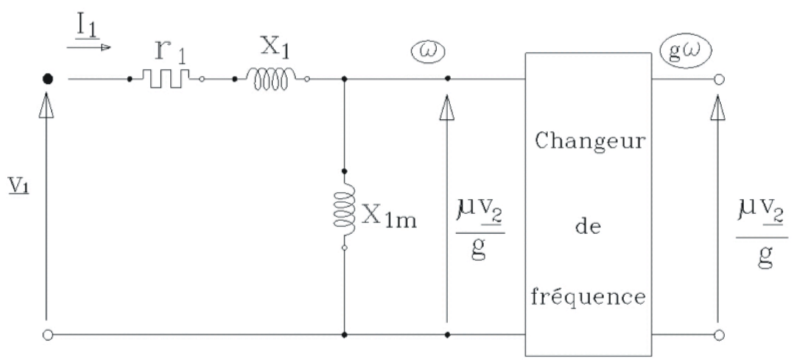
\includegraphics[scale=0.35]{ch5/image22.png}
	\captionof{figure}{ }
	\end{wrapfigure}
		On peut déduire la tension correspondante 
		\begin{equation}
		\underline{v_2} = jg\dfrac{X_{1m}}{\mu}I_1\sqrt{2}e^{j(g\omega t + \xi_I-\theta_0)}
		\end{equation}
		La pulsation des tensions rotoriques vaut $g\omega$. La machine est un \textbf{
		changeur de fréquence}. On définit alors le phaseur $\underline{V_2}$  :\\
		
		\begin{equation}
		\underline{V_2} = jg\dfrac{X_{1m}}{\mu}\underline{I_1}\qquad\Leftrightarrow\qquad 
		\dfrac{\mu\underline{V_2}}{g} = jX_{1m}\underline{I_1}
		\end{equation}
		et on en déduit le schéma équivalent. Le changeur de fréquence modifie la fréquence 
		de la tension, mais sans changer son amplitude.\\
		\danger Au synchronisme $\omega_r=\omega \Rightarrow g=0$, le champ est fixe par 
		rapport au stator : il ne peut y avoir de f.e.m. induite !
		
		\subsubsection{Alimentation par le rotor - Stator ouvert}
		Raisonnement similaire ! Notons que la pulsation des tensions et courants rotorique 
		doit valoir $g\omega$. Si c'est le cas, on obtient le schéma ci-dessous.
		\begin{center}
		\vspace{-3mm}
		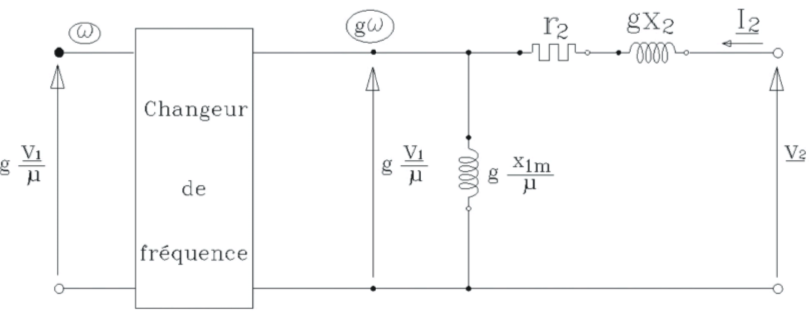
\includegraphics[scale=0.45]{ch5/image23.png}
		\captionof{figure}{ }
		\end{center}
		\newpage
		On peut transformer ce schéma en le schéma suivant, en multipliant les tensions par 
		$\mu/g$, les courants par $1/\mu$, les impédances par $\mu^2/g$ et en déplaçant le 
		changeur de fréquence.
		\begin{center}
		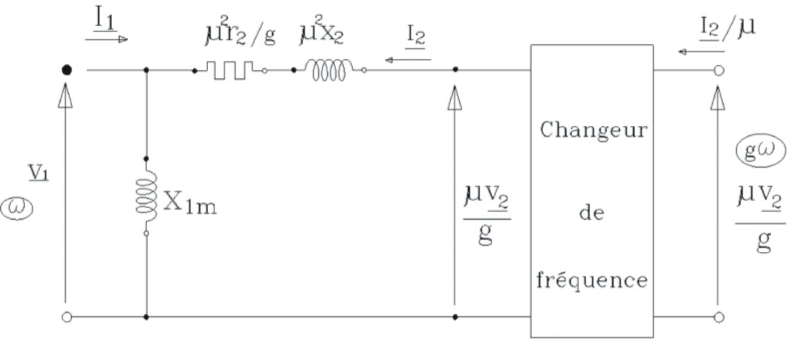
\includegraphics[scale=0.5]{ch5/image24.png}
		\captionof{figure}{ }
		\end{center}

		\subsubsection{Alimentation par le stator et le rotor}
		En superposant l'effet des courants statoriques et rotoriques, on obtient le 
		\textbf{schéma équivalent d'une machine asynchrone en rotation}.
		\begin{center}
		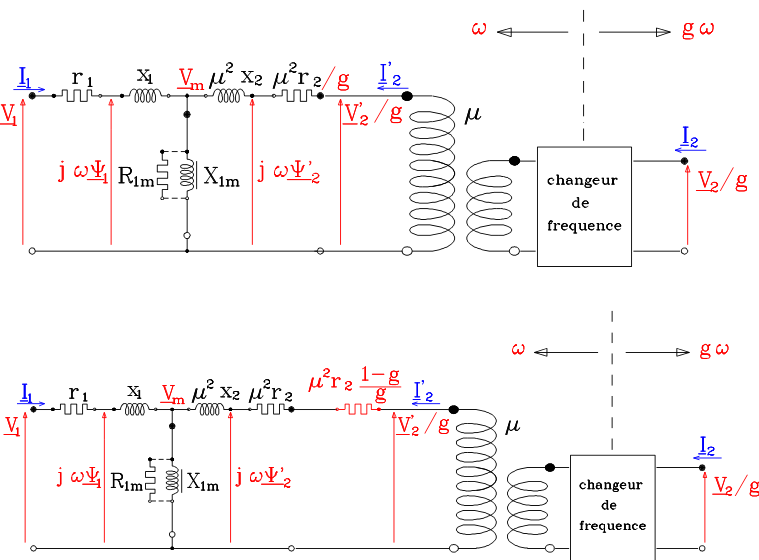
\includegraphics[scale=0.5]{ch5/image25.png}
		\captionof{figure}{ }
		\end{center}
		Deux grandes différences par rapport au schéma équivalent de la machine à 
		l'arrêt : le déphaseur est remplacé par un changeur de fréquence et une 
		résistance supplémentaire apparaît au rotor (voir plus bas).
		
		\newpage
		\subsubsection{Couples mécaniques}
		\begin{wrapfigure}[8]{l}{6.5cm}
		\vspace{-8mm}
		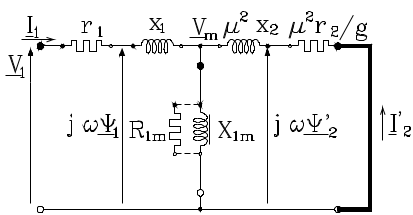
\includegraphics[scale=0.45]{ch5/image26.png}
		\captionof{figure}{ }
		\end{wrapfigure}
		Souvent, on court-circuite le rotor (moteur à cage) et l'on obtient le schéma 
		équivalent ci-contre; La puissance électrique appliquée au stator se décompose 
		en trois :
		\begin{enumerate}
		\item Pertes Joule au stator : $P_{pJ1} = 3r_1I_1^2$.
		\item Pertes magnétiques : $P_{pm} = 3V_m^2/R_{1m}$.
		\item Puissances transmise par l'entrefer au rotor : $P_{entr}$.
		\end{enumerate}
		On peut décomposer $P_{entr}$ en pertes Joules au rotor ($P_{pJ2} = 3r_2I_2^2$) 
		et en puissance électromagnétique brute à l'arbre ($P_{em} = C_{em}\Omega_r$). 
		L'analyse du schéma équivalent montre que cette puissance électromagnétique brute 
		doit valoir les pertes Joule dans la résistance supplémentaire $\mu^2[(1-g)g]r_2$.\\
		
		Après quelques calculs (page 5.52), on trouve pour le couple électromécanique brut :
		\begin{equation}
		C_{em} = \dfrac{p}{\omega}\dfrac{3r_2I_2^2}{g}
		\end{equation}
		Ce couple est proportionnel aux pertes Joule du rotor. Au synchronisme ($g=0$) 
		nous savons que $I_2=0$ et donc $C_{em}=0$. La machine n'est utilisable qu'en 
		dehors du synchronisme : machine \textbf{asynchrone}.



	\subsection{Diagramme des courants (ou du cercle)}
		\subsubsection{Préliminaires}
		Considérons un circuit $RX$, faisons varier $R$ et 0 à $\infty$ et notons la 
		tensions $V$ en fonction du courant. Lorsque $R$ varie, l'extrémité du phaseur 
		$\underline{I}$ décrit un lieu géométrique : demi-cercle.

		\subsubsection{Diagramme du cercle}
		Il indique la variation du courant \textbf{statorique} en fonction du 
		\textbf{glissement} lorsque la tension statorique est maintenue \textbf{constante}. 
		On maintient les impédances constantes\footnote{Attention néanmoins, $X_{1m}$ dépend 
		de l'état magnétique ($V_m$) et $r_2$ est fonction de la fréquence des courants 
		rotoriques (effet pelliculaire).}

			\begin{center}
		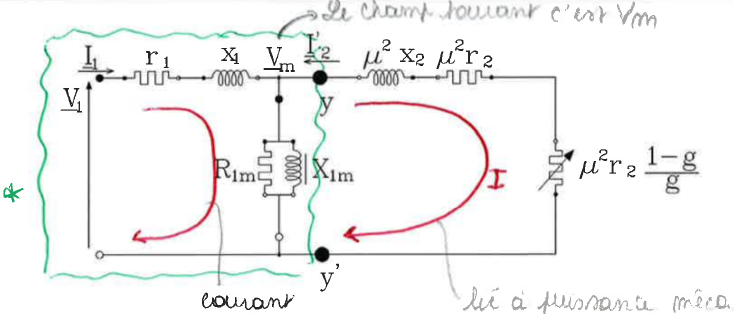
\includegraphics[scale=0.45]{ch5/image27.png}
		\captionof{figure}{ }
		\end{center}
		\newpage
		A droite, le courant magnétisant, à gauche le courant lié à la 
		puissance mécanique. Le champ tournant est bien $V_m$. On verra plus tard que la partie 
		entourée de vert peut être vu comme  un équivalent de Thévenin.\\
		Sur ce schéma, posons :
		\begin{itemize}
		\item[$\bullet$] $\underline{Z_{1m}} = R_{1m} // X_{1m} ;$ impédance de magnétisation 
		vue du stator
		\item[$\bullet$] $\underline{z_1} = r_1+jx_1$; impédance de dispersion du stator
		\item[$\bullet$] $\underline{z_2} = r_2+jx_2$; impédance de dispersion du rotor
		\item[$\bullet$] $\underline{z_2}' = \mu^2r_2+j\mu^2x_2 = r_2'+jx_2'$; impédance de 
		dispersion du rotor vue du 	stator.
		\end{itemize}
		Avec ces nouvelles définitions, on peut écrire l'équation de maille :
		\begin{equation}
		\underline{V_1} = \underline{z_1}\underline{I_1} + \underline{Z_{1m}}(\underline{I_1}+
		\underline{I_2}')
		\end{equation}
		Et donc
		\begin{equation}
		\underline{I_1} = \underbrace{\dfrac{\underline{V_1}}{\underline{z_1}+\underline{Z_{1m
		}}}}_{(*)}
		+ \underline{k_1}(-\underline{I_2}')
		\end{equation}
		où $(*)$ est le courant consommé au synchronisme (car $I_2=0, g=0$). En posant 
		\begin{equation}
		\underline{k_1} = \dfrac{\underline{Z_{1m}}}{\underline{z_1}+\underline{Z_{1m}}} = 
		k_1\angle\epsilon_1
		\end{equation}
		
						\begin{wrapfigure}[8]{r}{4.5cm}
		\vspace{-8mm}
		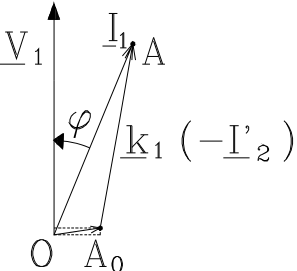
\includegraphics[scale=0.45]{ch5/image28.png}
		\captionof{figure}{ }
		\end{wrapfigure}
		le coefficient de couplage \textbf{généralisé} dont son module est proche de l'unité et 
		son argument faible (mais positif). Regardons le graphique de notre dernière relation. 
		$\underline{OA_0}$ représente $\underline{I_0}$, le courant statorique absorbé au 
		synchronisme (pas tout à fait -90$^\circ$ (car sert essentiellement à la magnétisation, 
		donc inductif) à cause des pertes Joules). Son amplitude est inversement proportionnel 
		(voir $(*)$) à la réactance de magnétisation. Pour améliorer le facteur de puissance du 
		courant, il faut réduire $I_0$ au maximum $\rightarrow$ augmenter $X_{1m} \rightarrow$ 
		réduire l'entrefer.\\
		
		Le phaseur $\underline{A_0A}$ est proportionnel au courant secondaire : il faut connaître 
		la variation en fonction du glissement. On applique Thévenin comme dit plus haut. On 
		peut successivement obtenir, après changements de variables 
		\begin{center}
		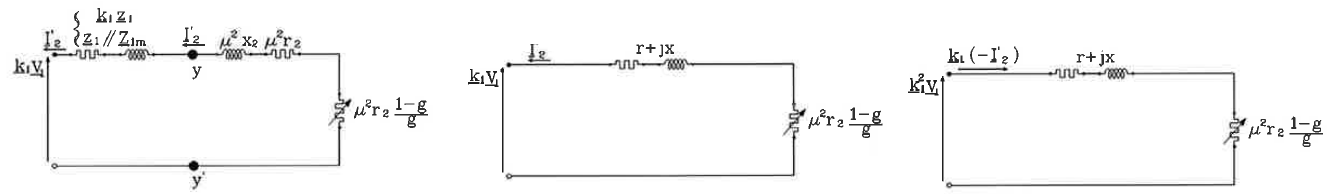
\includegraphics[scale=0.35]{ch5/image29.png}
		\captionof{figure}{ }
		\end{center}
		Sur le dernier schéma, en première approximation ($\underline{k_1}\approx 1$) 
		$\underline{z}$ vaut
		\begin{equation}
		\underline{z} = (r_1+\mu^2r_2) + j(x_1+\mu^2x_2)
		\end{equation}
		On construit alors le lieu	du point $A$ : 
		\begin{center}
		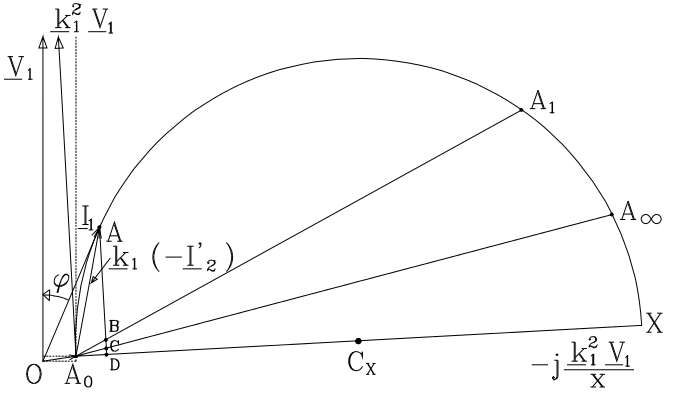
\includegraphics[scale=0.5]{ch5/image30.png}
		\captionof{figure}{ }
		\end{center}
		Sur ce graphe, $\underline{k_1}^2\underline{V_2}\approx\underline{V_1}$. L'amplitude 
		du courant dépend de $g$. Pour $g=1$, la résistance est celle du moteur à l'arrêt et 
		le courant ($I =V/R$) est 4.5* plus grand. On sait aussi que la machine à vide, à 
		part les frottements, tourne au synchronisme ($g=0$)(point $A_0$). Le point $A$ possède 
		un petit $g$ et un bon rendement car son $\cos\phi$ est proche de l'unité.
		
		On comprend alors que le lieu représente tous les $I$ possibles pour une résistance 
		variable (fonction de $g$).

		\textsc{A compléter avec les notes de labo. Éclaircir la dépendance en $g$.}
		
		
		
	\subsection{Caractéristique mécanique $C_{em} = f(\Omega_r)$ ou $C_{em} = f(g)$}
	On peut déduire la caractéristique du diagramme du cercle complété pour les glissements 
	négatifs (fonctionnement en génératrice, le rotor tourne plus vite que le champ tournant) en 
	"fermant le cercle".\\
	On distingue trois zones de fonctionnement :
	\begin{description}
	\item[Moteur] Entre $A_1$ et $A_0$ : le couple au démarrage doit être assez élevé pour faire 
	bouger la charge. La charge a généralement une caractéristique positive.
	\item[Freinage] Entre $A_\infty$ et $A_1$, la machine tourne en sens inverse du champ tournant.
	\item[Génératrice] Demi-cercle symétrique ("négatif) entre $A_\infty$ et$ A_0$.
	\end{description}
			\begin{center}
		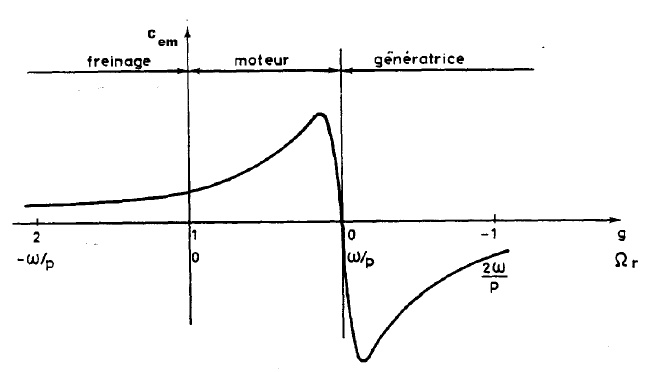
\includegraphics[scale=0.4]{ch5/image31.png}
		\captionof{figure}{ }
		\end{center}



\section{Le moteur asynchrone en cage d’écureuil en régime}














	
	
	
	
	
	
	
	
	
	
	